\documentclass[14pt]{beamer}

\mode<presentation>{ \usetheme{Madrid}

% To remove the navigation symbols from the bottom of all slides uncomment next line
\setbeamertemplate{navigation symbols}{}
\date{}
\title{}
\author{}

%to get rid of footer entirely uncomment next line
\setbeamertemplate{footline}{}
}

\usepackage{geometry}
\usepackage{multirow}
\usepackage{adjustbox}
\usepackage{multicol}
\setlength{\columnsep}{0.1cm}

\usepackage{tikz}
\usetikzlibrary{shapes, backgrounds}

\usepackage{bbding}
\usepackage{rotating}
\usepackage{xcolor}

%\usepackage{tkz-berge} %cool grid
\usepackage{pgfplots} %pics

\usepackage{graphicx} % Allows including images
\usepackage{
	booktabs
} % Allows the use of \toprule, \midrule and \bottomrule in tables
\usepackage{mathtools}

\newcommand{\R}{\mathbb{R}}
\newcommand{\Z}{\mathbb{Z}}
\newcommand{\N}{\mathbb{N}}
\newcommand{\e}{\varepsilon}

\newcommand{\p}{% \pause
}

% simple environrment for enumerate, easier to read
\setbeamertemplate{enumerate items}[default]

%%%%%%%%%%%%%%%%%%%%%%

% to use colours easily
\definecolor{verde}{rgb}{0, .7, 0}
\definecolor{rosa}{rgb}{1, 0, 1}
\definecolor{naranja}{rgb}{1, .5, 0.1}
\newcommand{\azul}[1]{{\color{blue} #1}}
\newcommand{\rojo}[1]{{\color{red} #1}}
\newcommand{\verde}[1]{{\color{verde} #1}}
\newcommand{\rosa}[1]{{\color{rosa} #1}}
\newcommand{\naranja}[1]{{\color{naranja} #1}}
\newcommand{\violeta}[1]{{\color{violet} #1}}

% box in red and blue in math and outside of math
\newcommand{\cajar}[1]{\boxed{\mbox{\rojo{ #1}}}}
\newcommand{\majar}[1]{\boxed{\rojo{ #1}}}
\newcommand{\cajab}[1]{\boxed{\mbox{\azul{ #1}}}}
\newcommand{\majab}[1]{\boxed{\azul{ #1}}}

\newcommand{\setsize}[1]{\fontsize{#1}{#1}\selectfont} %allows you to change the font size. The default size of this document is 14. To change the font size of the whole slide, place this at the beginning of the slide. To change the size of only a portion of the text to size 12, you can do the following { \setsize{12} Your text. }.

\setbeamerfont{frametitle}{size=\fontsize{15}{15}\selectfont}
\setbeamerfont{block title}{size=\fontsize{14}{14}\selectfont}

\newcommand{\smallerfont}{\setsize{13}} %place this at the beginning of a slide to set the font size of the entire slide to 13.

%===========================

% Preamble just for this file

%===========================

\newcommand{\erf}{\operatorname{erf}}
\newcommand{\vv}{\vspace{.2cm}}

%===================================================
\begin{document}
	%===================================================

	%----------------------------------------------------------------------------------------

	%	Integration by substitution

	%----------------------------------------------------------------------------------------

	%------------------------------

	%QUESTION_INFO: {"unit":9,"question":0,"title":"Warm up","images":[]}
	\begin{frame}[t]
		\frametitle{Warm up}

		Calculate
		\[
			\int \frac{\sin \sqrt{x}}{\sqrt{x}}\, dx
		\]

		\emph{Hint:} Use the substitution $\displaystyle u=\sqrt{x}$.
	\end{frame}

	%------------------------------

	%QUESTION_INFO: {"unit":9,"question":1,"title":"Computation practice: integration by substitution","images":[]}
	\begin{frame}[t]
		\frametitle{Computation practice: integration by substitution}

		Use substitutions to compute:
		\begin{multicols}{2}
			\begin{enumerate}
				\item $\displaystyle \int \frac{\sin \sqrt{x}}{\sqrt{x}}dx$
					\vspace{.2cm}

				\item $\displaystyle \int e^{x}\cos \left(e^{x}\right) dx$
					\vspace{.2cm}

				\item $\displaystyle \int \cot x \, dx$
					\vspace{.2cm}

				\item $\displaystyle \int x^{2}\sqrt{x+1}\, dx$
					\vspace{.2cm}
				% \pause

				\item $\displaystyle \int \frac{e^{2x}}{\sqrt{e^{x}+ 1}}\, dx$
					\vspace{.2cm}

				\item $\displaystyle \int \frac{\left( \ln \ln x \right)^{2}}{ x \ln x}\,
					dx$
					\vspace{.2cm}

				\item $\displaystyle \int x e^{-x^2}\, dx$
					\vspace{.2cm}

				\item $\displaystyle \int e^{-x^2}\, dx$
					\vspace{.2cm}
			\end{enumerate}
		\end{multicols}
	\end{frame}
	%------------------------------

	%QUESTION_INFO: {"unit":9,"question":2,"title":"Definite integral via substitution","images":[]}
	\begin{frame}
		\fontsize{13}{13}\selectfont
		\frametitle{Definite integral via substitution}

		This final answer is right, but the write-up is WRONG. Why?
		\vfill

		Calculate $\displaystyle I = \int_{0}^{2}\sqrt{x^{3}+1}\; x^{2}dx$
		\begin{block}{Wrong answer}
			Substitution: $\displaystyle u = x^{3}+1, \; du=3x^{2}dx$.
			\begin{align*}
				I \; & = \; \frac{1}{3}\int_{0}^{2}\sqrt{x^{3}+1}\; (3x^{2}dx)                             &  & = \; \frac{1}{3}\int_{0}^{2}u^{1/2}\; du                             \\
				     & = \; \frac{1}{3}\; \frac{2}{3}\; \left. u^{3/2}\right\vert_{0}^{2}                  &  & = \; \left. \frac{1}{9}\left(x^{3}+1\right)^{2/3}\right\vert_{0}^{2} \\
				     & = \; \frac{2}{9}\left( 2^{3}+ 1 \right)^{3/2}- \frac{2}{9}\left( 0 + 1\right)^{3/2} &  & = \; \frac{52}{9}
			\end{align*}
		\end{block}
	\end{frame}
	%------------------------------

	%QUESTION_INFO: {"unit":9,"question":3,"title":"Integral of products of $\\sin$ and $\\cos$","images":[]}
	\begin{frame}[t]
		\fontsize{13}{13}\selectfont
		\frametitle{Integral of products of $\sin$ and $\cos$}
		We want to compute
		\vspace{-.5cm}
		\[
			I = \int \sin^{3}x \cos^{2}x \, dx
		\]

		\begin{enumerate}
			\item Attempt the substitution $\displaystyle u = \sin x$

			\item Attempt the substitution $\displaystyle u = \cos x$

			\item One worked better than the other. Which one? Why? \\ Finish the
				problem.
			% \pause

			\item Assume we want to compute
				\[
					\int \sin^{n}x \cos^{m}x \, dx
				\]
				When will the substitution $\displaystyle u = \sin x$ be helpful? \\
				When will the substitution $\displaystyle u = \cos x$ be helpful?
		\end{enumerate}
	\end{frame}
	%------------------------------

	%QUESTION_INFO: {"unit":9,"question":4,"title":"Odd functions","images":[]}
	\begin{frame}[t]
		\fontsize{13}{13}\selectfont
		\frametitle{Odd functions}

		\begin{block}{Theorem}
			Let $f$ be a continuous function. Let $a >0$. IF $f$ is odd, THEN
			\[
				\int_{-a}^{a}f(x) dx = 0
			\]
		\end{block}

		% \pause

		\begin{enumerate}
			\item Write down the definition of ``odd function".

			\item Draw a picture to interpret the theorem geometrically.

			\item Prove the theorem!

				\emph{Hint:} Write the integral as sum of two pieces. Use a substitution
				to show that one of the two pieces equals minus the other.
		\end{enumerate}
	\end{frame}
	%------------------------------

	%----------------------------------------------------------------------------------------

	%	Integration by parts

	%----------------------------------------------------------------------------------------

	%------------------------------

	%QUESTION_INFO: {"unit":9,"question":5,"title":"Computation practice: Integration by parts","images":[]}
	\begin{frame}[t]
		\frametitle{Computation practice: Integration by parts}

		Use integration by parts (possibly in combination with other methods) to
		compute:
		\begin{multicols}{2}
			\begin{enumerate}
				\item $\displaystyle \int x e^{-2x}dx$
					\vspace{.2cm}

				\item $\displaystyle \int x^{2}\sin x \, dx$
					\vspace{.2cm}

				\item $\displaystyle \int \ln x \, dx$
					\vspace{.2cm}

				\item $\displaystyle \int \sin \sqrt{x}\, dx$
					\vspace{.2cm}
				% \pause

				\item $\displaystyle \int x \arctan x \, dx$
					\vspace{.2cm}

				\item $\displaystyle \int x^{2}\arcsin x \, dx$
					\vspace{.2cm}

				\item $\displaystyle \int e^{\cos x}\sin^{3}x \, dx$
					\vspace{.2cm}

				\item $\displaystyle \int e^{ax}\sin (bx) dx$
					\vspace{.2cm}
			\end{enumerate}
		\end{multicols}
	\end{frame}
	%------------------------------

	%QUESTION_INFO: {"unit":9,"question":6,"title":"Persistence","images":[]}
	\begin{frame}[t]
		\frametitle{Persistence}
		Compute
		\begin{multicols}{2}
			\begin{itemize}
				\item $\displaystyle \int_{1}^{e}\left( \ln x \right)^{3}dx$
					% \pause
					\vspace{.2cm}

				\item $\displaystyle \int_{1}^{e}\left( \ln x \right)^{10}dx$
			\end{itemize}
		\end{multicols}
		% \pause
		There is a more efficient approach. Call
		\[
			I_{n}= \int_{1}^{e}\left( \ln x \right)^{n}dx
		\]
		Use integration by parts on $I_{n}$. You will get an equation with $I_{n}$ and
		$I_{n-1}$. Now solve the previous questions.

		\vfill
		\hfill \href{https://oeis.org/}{\beamergotobutton{OEIS}}
	\end{frame}

	%------------------------------

	%QUESTION_INFO: {"unit":9,"question":7,"title":"Integrals from a graph","images":["G22b.svg","G22b.png","G22a.svg","G22a.png","G22.svg","G22.png"]}
	\begin{frame}[t]
		\frametitle{Integrals from a graph}

		\begin{columns}
			\begin{column}{.7\textwidth}
				\begin{center}
					\only<1>{
					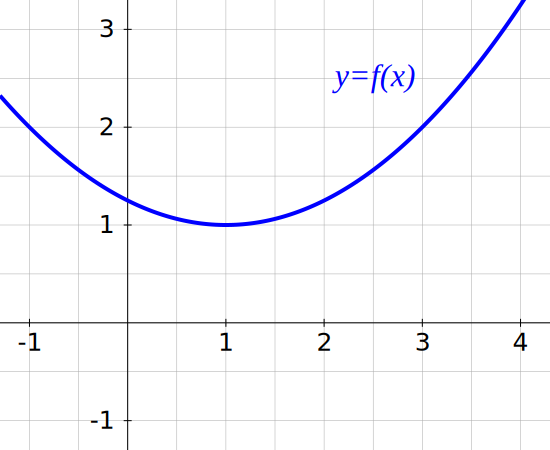
\includegraphics[scale=.4]{G22}
					} \only<2>{
					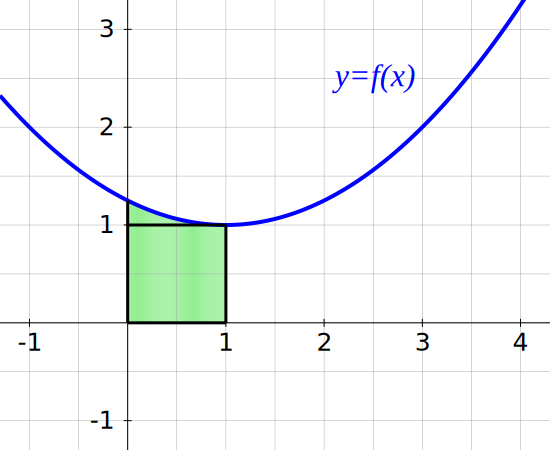
\includegraphics[scale=.4]{G22a}
					} \only<3>{
					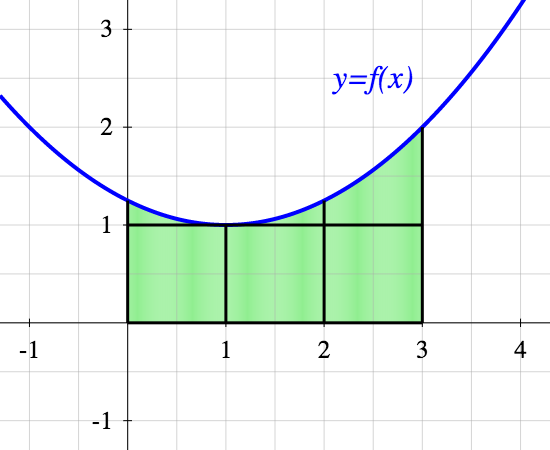
\includegraphics[scale=.4]{G22b}
					}
				\end{center}
			\end{column}

			\begin{column}{.32\textwidth}
				Estimate:
				\begin{enumerate}
					\item $\displaystyle \int_{0}^{1}f(x) dx$

					\item $\displaystyle \int_{0}^{1}f'(x) dx$

					\item $\displaystyle \int_{0}^{3}x \, f'(x) dx$

					\item $\displaystyle \int_{0}^{1}f(3x) dx$
				\end{enumerate}
			\end{column}
		\end{columns}
	\end{frame}
	%------------------------------

	%QUESTION_INFO: {"unit":9,"question":8,"title":"The error function","images":[]}
	\begin{frame}[t]
		\frametitle{The error function}

		The following function is tabulated.
		\[
			{\Large E(x) = \int_0^x e^{-t^2} dt}.
		\]
		Write the following quantities in terms of $E$:

		\begin{multicols}{2}
			\begin{enumerate}
				\item $\displaystyle \int_{1}^{2}e^{-t^2}dt$

					\vspace{.2cm}

				\item $\displaystyle \int_{0}^{x}t^{2}e^{-t^2}dt$

					\vspace{.2cm}

				\item $\displaystyle \int_{0}^{x}e^{-2t^2}dt$

					\vspace{.2cm}
				% \pause

				\item $\displaystyle \int_{0}^{1}e^{-t^2+6t}dt$

					\vspace{.2cm}

				\item $\displaystyle \int_{x_1}^{x_2}e^{-\frac{(t- \mu)^{2}}{\sigma^{2}}}
					dt$

					\vspace{.2cm}

				\item $\displaystyle \int_{1}^{2}\frac{e^{-t}}{\sqrt{t}}dt$
			\end{enumerate}
		\end{multicols}
	\end{frame}
	%------------------------------

	%QUESTION_INFO: {"unit":9,"question":9,"title":"Exp-trig antiderivative","images":[]}
	\begin{frame}[t]
		\frametitle{Exp-trig antiderivative}

		We want to compute
		\[
			I = \int e^{ax}\sin (bx) \; dx
		\]
		\begin{itemize}
			\item Try once integration by parts choosing $\displaystyle u = e^{ax}$.
				Stop.

			\item Go back to $I$. Now try integration by parts once choosing
				$\displaystyle u = \sin (bx)$ instead. Stop.

			\item Look at what you did. Think.
		\end{itemize}
	\end{frame}
	%------------------------------

	%----------------------------------------------------------------------------------------

	%	Integration of products of trigonometric functions

	%----------------------------------------------------------------------------------------

	%------------------------------

	%QUESTION_INFO: {"unit":9,"question":10,"title":"Practice: Integrals with trigonometric functions","images":[]}
	\begin{frame}[t]
		\fontsize{13}{13}\selectfont
		\frametitle{Practice: Integrals with trigonometric functions}

		Compute the following antiderivatives. (Once you get them to a form from where
		you see a path to finish them, even if long, you may stop.)

		\begin{multicols}{2}
			\begin{enumerate}
				\item $\displaystyle \int \sin^{10}x \cos x \ dx$
					\vspace{.2cm}

				\item $\displaystyle \int \sin^{10}x \cos^{7}x \, dx$
					\vspace{.2cm}

				\item $\displaystyle \int e^{\cos x}\cos x \sin^{3}x \, dx$
					\vspace{.2cm}

				\item $\displaystyle \int \cos^{2}x \, dx$
					\vspace{.2cm}

				\item $\displaystyle \int \cos^{4}x \, dx$
					\vspace{.2cm}

				\item $\displaystyle \int \csc x \, dx$
					\vspace{.2cm}
			\end{enumerate}
		\end{multicols}

		\vspace{-.5cm}
		{\fontsize{10}{10}\selectfont \begin{block}{ \fontsize{12}{12}\selectfont Useful trig identities}\vspace{-.5cm} \begin{align*}\large&\sin^{2}x + \cos^{2}x = 1&\sin^{2}x&= \frac{1 - \cos (2x)}{2}\\&\tan^{2}x + 1 = \sec^{2}x&\cos^{2}x&= \frac{1 + \cos (2x)}{2}\end{align*}\end{block} }
	\end{frame}
	%------------------------------

	%QUESTION_INFO: {"unit":9,"question":11,"title":"Integral of products of secant and tangent","images":[]}
	\begin{frame}[t]
		\frametitle{Integral of products of secant and tangent}

		To integrate
		\[
			\int \sec^{n}x \tan^{m}x \, dx
		\]
		\begin{itemize}
			\item If \boxed{\phantom{spacespace}}, then use the substitution $\displaystyle
				u = \tan x$.

			\item If \boxed{\phantom{spacespace}}, then use the substitution $\displaystyle
				u = \sec x$.
		\end{itemize}

		\vfill

		{\fontsize{13}{13}\selectfont \emph{Hint:} You will need \begin{itemize}\begin{multicols}{2}\item $\displaystyle \frac{d}{dx}\left[ \tan x \right] = \ldots$ \item $\displaystyle \frac{d}{dx}\left[ \sec x \right] = \ldots$\end{multicols}

		\item The trig identity involving $\sec$ and $\tan$\end{itemize} }
	\end{frame}
	%------------------------------

	%QUESTION_INFO: {"unit":9,"question":12,"title":"A reduction formula","images":[]}
	\begin{frame}[t]
		\fontsize{13}{13}\selectfont
		\frametitle{A reduction formula}

		Let $\displaystyle I_{n}= \int_{0}^{2\pi}\sin^{n}x \, dx$.
		\vspace{.3cm}

		\begin{enumerate}
			\item Compute $I_{0}$ and $I_{1}$.
				\vspace{.3cm}

			\item Write an equation for $\displaystyle I_{n}$ in terms of $\displaystyle
				I_{n-2}$. This is called a reduction formula.
				\vspace{.3cm}

				\emph{Hint:} Starting with $I_{n}$, use integration by parts once. \\ Then
				use $\displaystyle \sin^{2}x + \cos^{2}x = 1$ to rewrite the new integral
				in terms of $\displaystyle I_{n}$ and $\displaystyle I_{n-2}$.
				\vspace{.3cm}

			\item Write a a formula for $I_{n}$ for all natural numbers $n$.

			%\DS{I_8 = \frac{35}{64} \pi}.
		\end{enumerate}
	\end{frame}
	%------------------------------

	%QUESTION_INFO: {"unit":9,"question":13,"title":"A different kind of substitution","images":[]}
	\begin{frame}[t]
		\frametitle{A different kind of substitution}

		Calculate
		\[
			\int_{0}^{1}\sqrt{1 - x^{2}}\; dx
		\]
		using the substitution
		\[
			\begin{cases}
				x = \sin \theta \\
				dx = ??
			\end{cases}
		\]
	\end{frame}
	%------------------------------

	%----------------------------------------------------------------------------------------

	%	Integration of rational functions

	%----------------------------------------------------------------------------------------

	%------------------------------

	%QUESTION_INFO: {"unit":9,"question":14,"title":"Rational integrals","images":[]}
	\begin{frame}[t]
		\fontsize{13}{13}\selectfont
		\frametitle{Rational integrals}

		\begin{enumerate}
			\item Calculate $\displaystyle \int \frac{1}{x+a}\, dx$
				\vspace{.2cm}

			\item Reduce to common denominator \, $\displaystyle \frac{2}{x}- \frac{3}{x+3}$
				\vspace{.2cm}

			\item Calculate $\displaystyle \int \frac{-x + 6}{x^{2}+ 3x}\, dx$
				\vspace{.2cm}

			\item Calculate $\displaystyle \int \frac{1}{x^{2}+ 3x}\, dx$
				\vspace{.2cm}

			\item Calculate $\displaystyle \int \frac{1}{x^{3}-x}\, dx$
		\end{enumerate}
	\end{frame}
	%-------------------------------

	%QUESTION_INFO: {"unit":9,"question":15,"title":"Repeated factors","images":[]}
	\begin{frame}[t]
		\fontsize{13}{13}\selectfont
		\frametitle{Repeated factors}

		\begin{enumerate}
			\item Calculate $\displaystyle \int \frac{1}{(x+1)^{n}}\, dx$ \quad for $n
				>1$
				\vspace{.2cm}

			\item Calculate $\displaystyle \int \frac{(x+1) - 1}{(x+1)^{2}}\, dx$
				\vspace{.2cm}

			\item Calculate $\displaystyle \int \frac{2x + 6}{(x+1)^{2}}\, dx$
				\vspace{.2cm}

			\item Calculate $\displaystyle \int \frac{x^{2}}{(x+1)^{3}}\, dx$
		\end{enumerate}
	\end{frame}
	%-------------------------------

	%QUESTION_INFO: {"unit":9,"question":16,"title":"Irreducible quadratics","images":[]}
	\begin{frame}[t]
		\fontsize{13}{13}\selectfont
		\frametitle{Irreducible quadratics}

		\begin{enumerate}
			\item Calculate $\displaystyle \int \frac{1}{x^{2}+ 1}\, dx$ and $\displaystyle
				\int \frac{x}{x^{2}+1}\, dx$.
				\vspace{.2cm}

				\emph{Hint:} These two are very short.
				\vspace{.2cm}

			\item Calculate $\displaystyle \int \frac{2x+ 3}{x^{2}+ 1}\, dx$
				\vspace{.2cm}

			\item Calculate $\displaystyle \int \frac{x^{2}}{x^{2}+ 1}\, dx$
				\vspace{.2cm}

			\item Calculate $\displaystyle \int \frac{x}{x^{2}+ x + 1 }\, dx$
				\vspace{.2cm}

				\emph{Hint:} Complete the square in the denominator and use a substitution
				to transform into one of the previous ones.
		\end{enumerate}
	\end{frame}
	%-------------------------------

	%QUESTION_INFO: {"unit":9,"question":17,"title":"Repeated quadratics","images":[]}
	\begin{frame}[t]
		\frametitle{Repeated quadratics}

		\begin{enumerate}
			\item Calculate
				\[
					\frac{d}{dx}\left[ \arctan x \right], \quad \quad \frac{d}{dx}\left[ \frac{x}{1+x^{2}}
					\right].
				\]

			\item Use the previous answer to calculate
				\[
					\int \frac{1}{\left(1+x^{2}\right)^{2}}\; dx
				\]
		\end{enumerate}
	\end{frame}
	%-------------------------------

	%QUESTION_INFO: {"unit":9,"question":18,"title":"The integral of secant","images":[]}
	\begin{frame}[t]
		\frametitle{The integral of secant}

		Compute
		\[
			\int \sec x \, dx
		\]
		using the substitution $\displaystyle u = \sin x$.
	\end{frame}
	%-------------------------------

	%QUESTION_INFO: {"unit":9,"question":19,"title":"Messier rational functions","images":[]}
	\begin{frame}[t]
		\frametitle{Messier rational functions}

		\begin{enumerate}
			\item How could we compute an integral of the form
				\[
					\int \frac{\text{polynomial}}{(x+1)^{3}(x+2)}\, dx \; ?
				\]

			\item How could we compute an integral of the form
				\[
					\int \frac{\text{polynomial}}{x^{4}(x+1)^{3}(x+2)(x^{2}+1)(x^{2}+4)}\,d
					x \; ?
				\]
		\end{enumerate}
	\end{frame}
	%-------------------------------

	%------------------------------

	%-----------------------------
\end{document}
%-----------------------------

%-----------------------------